\section{离开鞍点}
\label{sec:saddle-escape}

迭代点已经到了梯度很小的鞍点邻域，怎样离开？回答取决于手里有什么信息。知道一个负曲率方向时，可以沿它走一步；只有梯度时，可以给迭代点一点随机扰动，让梯度下降自己放大不稳定的分量；有二次模型时，可以保留模型的不定性，让子问题自己走到负曲率的一侧。三种机制各有条件，都不能把严格鞍点的结论直接搬到退化驻点上。

\subsection{负曲率步}
\label{sec:saddle-nc-step}

上一节的检测给出了单位向量$\bm{v}$，满足$\bm{v}^\top\bm{H}\bm{v}\leq-\gamma$。站在山口上，这是一条明确的下坡路。问题是这样走一步能保证下降多少，步长又该取多大。

\paragraph{为什么要控制Hessian的变化}
二阶模型沿$\bm{v}$的预测是$-\tfrac12\gamma\alpha^2$，步长越大下降越多，但这个预测不可能一直成立。模型只在局部有效，走远了Hessian会变。例中沿$x_1$轴，
\[
 f(\alpha,0)=\frac14\bigl(\alpha^2-1\bigr)^2.
\]

$\alpha=1$处到达谷底，$\alpha=\sqrt2$处函数值回到$1/4$，再往前目标反而高于起点。所以负曲率方向不能无限延长，步长要受Hessian变化速度的约束，这个速度就是$M$。下面的引理给出二阶模型的误差。

\begin{lemma}[三次上界]
 \label{lem:saddle-cubic}
 设$\nabla^2f$在凸集$\bm{U}$上是$M$-Lipschitz的，$\bm{x}$与$\bm{x}+\bm{p}$都在$\bm{U}$中。记$\bm{g}=\nabla f(\bm{x})$，$\bm{H}=\nabla^2f(\bm{x})$，则
 \begin{equation}
  \Bigl\lvert f(\bm{x}+\bm{p})-f(\bm{x})-\langle\bm{g},\bm{p}\rangle-\frac12\bm{p}^\top\bm{H}\bm{p}\Bigr\rvert
  \leq\frac{M}{6}\lVert\bm{p}\rVert_2^3.
  \label{eq:saddle-cubic}
 \end{equation}
\end{lemma}

\begin{proof}
 令$\phi(s)=f(\bm{x}+s\bm{p})$，$s\in[0,1]$。由积分余项形式的Taylor公式，
 \[
  \phi(1)=\phi(0)+\phi'(0)+\int_0^1(1-s)\phi''(s)\,\mathrm{d}s.
 \]

 其中$\phi'(0)=\langle\bm{g},\bm{p}\rangle$。又因为$\int_0^1(1-s)\,\mathrm{d}s=\tfrac12$，二次项可以写进同一个积分，得到
 \[
  f(\bm{x}+\bm{p})-f(\bm{x})-\langle\bm{g},\bm{p}\rangle-\frac12\bm{p}^\top\bm{H}\bm{p}
  =\int_0^1(1-s)\bigl(\phi''(s)-\phi''(0)\bigr)\,\mathrm{d}s.
 \]

 $\phi$的二阶导数是Hessian沿$\bm{p}$的二次型，由Lipschitz条件，
 \[
  \lvert\phi''(s)-\phi''(0)\rvert
  =\bigl\lvert\bm{p}^\top\bigl(\nabla^2f(\bm{x}+s\bm{p})-\bm{H}\bigr)\bm{p}\bigr\rvert
  \leq Ms\lVert\bm{p}\rVert_2^3.
 \]

 代入并用$\int_0^1(1-s)s\,\mathrm{d}s=\tfrac16$，即得式~\eqref{eq:saddle-cubic}。
\end{proof}

\paragraph{选符号，定步长}
梯度不为零时，$\bm{v}$和$-\bm{v}$的曲率相同，一阶项却相反。所以先选符号，使一阶项不起反作用。下面的定理给出一步的下降量。

\begin{theorem}[负曲率步的下降]
 \label{thm:saddle-nc-step}
 设单位向量$\bm{v}$满足$\bm{v}^\top\bm{H}\bm{v}\leq-\gamma<0$和$\langle\bm{g},\bm{v}\rangle\leq0$，引理~\ref{lem:saddle-cubic}的条件对$\bm{p}=\alpha\bm{v}$成立。则对$\alpha>0$，
 \begin{equation}
  f(\bm{x}+\alpha\bm{v})\leq f(\bm{x})-\frac{\gamma}{2}\alpha^2+\frac{M}{6}\alpha^3.
  \label{eq:saddle-nc-bound}
 \end{equation}
 取$\alpha=2\gamma/M$时，
 \begin{equation}
  f(\bm{x}+\alpha\bm{v})\leq f(\bm{x})-\frac{2\gamma^3}{3M^2}.
  \label{eq:saddle-nc-decrease}
 \end{equation}
\end{theorem}

\begin{proof}
 由式~\eqref{eq:saddle-cubic}取$\bm{p}=\alpha\bm{v}$，$\lVert\bm{p}\rVert_2=\alpha$，得到
 \[
  f(\bm{x}+\alpha\bm{v})\leq f(\bm{x})+\alpha\langle\bm{g},\bm{v}\rangle+\frac{\alpha^2}{2}\bm{v}^\top\bm{H}\bm{v}+\frac{M}{6}\alpha^3.
 \]

 由$\langle\bm{g},\bm{v}\rangle\leq0$和$\bm{v}^\top\bm{H}\bm{v}\leq-\gamma$，即得式~\eqref{eq:saddle-nc-bound}。右端作为$\alpha$的函数，对$\alpha$求导得$-\gamma\alpha+\tfrac12M\alpha^2$，在$\alpha=2\gamma/M$处取到最小。代入得
 \[
  -\frac{\gamma}{2}\cdot\frac{4\gamma^2}{M^2}+\frac{M}{6}\cdot\frac{8\gamma^3}{M^3}
  =-\frac{2\gamma^3}{M^2}+\frac{4\gamma^3}{3M^2}
  =-\frac{2\gamma^3}{3M^2}.
 \]
\end{proof}

下降量只依赖负曲率的大小和Hessian的变化速度，与梯度多小无关。这正是它补上梯度步短板的地方：梯度步的保证是$\lVert\bm{g}\rVert_2^2/(2L)$，鞍点附近这个量几乎为零。

例中在原点取$\bm{v}=(1,0)$，$\gamma=1$，$M=6$，步长$\alpha=1/3$。定理保证的下降是
\[
 \frac{2\gamma^3}{3M^2}=\frac{1}{54}\approx0.0185.
\]
实际下降是
\[
 f(\bm{0})-f\bigl(\tfrac13,0\bigr)=\frac14-\frac{16}{81}\approx0.0525.
\]
图~\ref{fig:saddle-nc-slice}(a)沿$x_1$轴比较目标（蓝）、二次模型（绿）和三次上界（紫）。三次上界在$\bm{U}$内从上方盖住目标，绿点$\alpha=1/3$是上界的最低点，这个步长比实际的最好步长$\alpha=1$保守得多。

\begin{BookInlineFigure}
  \centering
  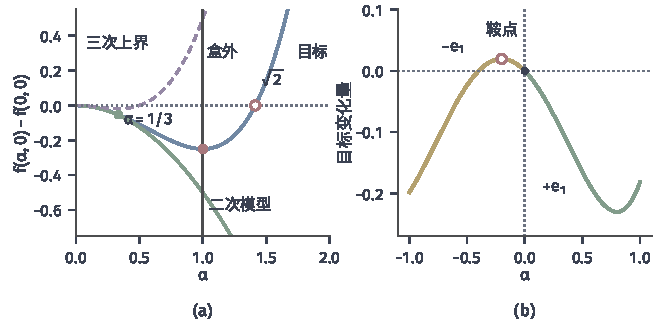
\includegraphics[width=112mm]{figures/05-optimization/02-smooth-optimization/matplotlib/saddle-nc-slice/figure.pdf}
  \caption{沿负曲率方向的一维截面。(a)原点沿$\bm{e}_1$：蓝线是目标减去$f(\bm{0})$，绿线是二次模型$-\alpha^2/2$，紫色虚线是三次上界$-\alpha^2/2+\alpha^3$，竖线是带形$\bm{U}$的边界。空心点$\alpha=\sqrt2$处目标回到起点的值。(b)从$(0.2,0)$出发沿$\pm\bm{e}_1$的目标变化，此处$\langle\bm{g},\bm{e}_1\rangle<0$。绿线一开始就下降，黄线先升到鞍点的高度才下降。}
  \label{fig:saddle-nc-slice}
\end{BookInlineFigure}

符号的作用见图~\ref{fig:saddle-nc-slice}(b)。在$(0.2,0)$处，梯度的第一个分量是$0.008-0.2=-0.192$，$+\bm{e}_1$满足$\langle\bm{g},\bm{v}\rangle<0$。朝$-\bm{e}_1$走，目标要先爬回鞍点才开始下降，一阶项抵消了曲率的好处。

\paragraph{不知道$M$时}
步长$2\gamma/M$要用到$M$，多数问题不知道它的值。这时可以回溯：从$\alpha_0$开始，不断折半，直到满足
\begin{equation}
 f(\bm{x}+\alpha\bm{v})\leq f(\bm{x})-\frac{\gamma}{4}\alpha^2.
 \label{eq:saddle-nc-backtrack}
\end{equation}

由式~\eqref{eq:saddle-nc-bound}，条件成立只需要
\[
 -\frac12\gamma\alpha^2+\frac16M\alpha^3\leq-\frac14\gamma\alpha^2,
\]
也就是$\alpha\leq3\gamma/(2M)$。折半回溯接受的步长因此不小于$\min\{\alpha_0,3\gamma/(4M)\}$，当$\alpha_0$足够大时，一步的下降不少于
\[
 \frac{\gamma}{4}\Bigl(\frac{3\gamma}{4M}\Bigr)^2=\frac{9\gamma^3}{64M^2}.
\]
例中取$\alpha_0=2$，$f(2,0)=9/4$被拒绝，$\alpha=1$时$f(1,0)=0\leq\tfrac14-\tfrac14$，被接受，一步到达谷底。

\paragraph{主要思想：梯度步和负曲率步交替}
梯度步在梯度大时有效，负曲率步在梯度小时仍然有效，两者正好互补。算法每轮先看梯度：梯度大就走梯度步；梯度小才花力气检测负曲率；两者都不能下降就停止。写成公式，
\begin{equation}
 \bm{x}^{(t+1)}=
 \begin{cases}
  \bm{x}^{(t)}-\dfrac{1}{L}\bm{g}^{(t)}, & \lVert\bm{g}^{(t)}\rVert_2>\varepsilon_g,\\
  \bm{x}^{(t)}+\dfrac{2\gamma^{(t)}}{M}\bm{v}^{(t)}, & \text{其他情形且检测到负曲率}.
 \end{cases}
 \label{eq:saddle-nc-update}
\end{equation}
其中单位向量$\bm{v}^{(t)}$的曲率是$-\gamma^{(t)}$，符号已经选定。$\varepsilon_g$和$\varepsilon_H$是梯度和曲率的容差，第~\ref{sec:saddle-stopping}节再讨论怎样取值。

\needspace{6\baselineskip}
\paragraph{变量}
算法要维护的量是：
\begin{itemize}
 \item $\bm{x}^{(t)}\in\mathbb{R}^n$：当前点；
 \item $\bm{g}^{(t)}\in\mathbb{R}^n$：当前梯度，每轮读取一次；
 \item $\bm{v}^{(t)}\in\mathbb{R}^n$，$\gamma^{(t)}>0$：只在梯度小的轮次计算的负曲率方向及其大小。
\end{itemize}

\paragraph{初始化}
选定$\bm{x}^{(0)}$、$L$、$M$和容差。例中$L=2$，$M=6$，$\varepsilon_g=0.1$，$\varepsilon_H=\sqrt{M\varepsilon_g}\approx0.775$，起点取在$x_2$轴上，并且用特征分解做检测：
\[
 \bm{x}^{(0)}=\begin{bmatrix}0\\1\end{bmatrix}.
\]

\paragraph{每轮更新}
第$t$轮依次执行以下步骤，直到第$3$步宣布停止。

\begin{enumerate}
 \item 计算$\bm{g}^{(t)}$。若$\lVert\bm{g}^{(t)}\rVert_2>\varepsilon_g$，由式~\eqref{eq:saddle-nc-update}走梯度步，进入下一轮。例中前$4$轮$x_1$一直是$0$，$x_2$每轮减半：
 \[
  \bm{x}^{(1)}=\begin{bmatrix}0\\0.5\end{bmatrix},\quad
  \bm{x}^{(2)}=\begin{bmatrix}0\\0.25\end{bmatrix},\quad
  \bm{x}^{(3)}=\begin{bmatrix}0\\0.125\end{bmatrix},\quad
  \bm{x}^{(4)}=\begin{bmatrix}0\\0.0625\end{bmatrix}.
 \]
 \item 否则检测负曲率。例中第$4$轮$\lVert\bm{g}^{(4)}\rVert_2=0.0625\leq0.1$，由式~\eqref{eq:saddle-example-derivatives}，
 \[
  \bm{H}^{(4)}=\operatorname{diag}(-1,1),\qquad\lambda_{\min}=-1<-\varepsilon_H.
 \]
 \item 若$\lambda_{\min}\geq-\varepsilon_H$，停止并返回$\bm{x}^{(t)}$。否则取$\bm{v}^{(t)}$为最小特征向量，$\gamma^{(t)}=-\lambda_{\min}$，选好符号，由式~\eqref{eq:saddle-nc-update}走负曲率步。例中第$4$轮$\langle\bm{g}^{(4)},\bm{e}_1\rangle=0$，取$\bm{v}=\bm{e}_1$，步长$1/3$，得到
 \[
  \bm{x}^{(5)}=\begin{bmatrix}1/3\\0.0625\end{bmatrix}.
 \]
\end{enumerate}

此后梯度已经变大，算法回到梯度步。表~\ref{tab:saddle-nc-run}列出全过程。第$9$轮$\lVert\bm{g}^{(9)}\rVert_2=0.060\leq0.1$，Hessian是$\operatorname{diag}(1.815,1)$，$\lambda_{\min}=1\geq-\varepsilon_H$，算法停止，最终得到$\bm{x}^{(9)}\approx(0.9686,0.0039)$。

\begin{BookInlineTable}
  \centering
  \begin{tabular}{@{}rccccl@{}}
    \toprule
    $t$ & $\bm{x}^{(t)}$ & $f$ & $\lVert\bm{g}^{(t)}\rVert_2$ & $\lambda_{\min}$ & 本轮动作\\
    \midrule
    $0$ & $(0,\ 1)$ & $0.7500$ & $1.000$ & $-1$ & 梯度步\\
    $1$ & $(0,\ 0.5)$ & $0.3750$ & $0.500$ & $-1$ & 梯度步\\
    $2$ & $(0,\ 0.25)$ & $0.2813$ & $0.250$ & $-1$ & 梯度步\\
    $3$ & $(0,\ 0.125)$ & $0.2578$ & $0.125$ & $-1$ & 梯度步\\
    $4$ & $(0,\ 0.0625)$ & $0.2520$ & $0.063$ & $-1$ & 负曲率步\\
    $5$ & $(0.3333,\ 0.0625)$ & $0.1995$ & $0.303$ & $-0.667$ & 梯度步\\
    $6$ & $(0.4815,\ 0.0313)$ & $0.1480$ & $0.371$ & $-0.305$ & 梯度步\\
    $7$ & $(0.6664,\ 0.0156)$ & $0.0774$ & $0.371$ & $0.332$ & 梯度步\\
    $8$ & $(0.8516,\ 0.0078)$ & $0.0189$ & $0.234$ & $1$ & 梯度步\\
    $9$ & $(0.9686,\ 0.0039)$ & $0.0010$ & $0.060$ & $1$ & 停止\\
    \bottomrule
  \end{tabular}
  \caption{梯度步与负曲率步在目标~\eqref{eq:saddle-example}上的运行。$\varepsilon_g=0.1$，$\varepsilon_H\approx0.775$，$\lambda_{\min}$是Hessian~\eqref{eq:saddle-example-derivatives}的最小特征值，第$8$、$9$轮第一个对角元已大于$1$，最小特征值取到$1$。}
  \label{tab:saddle-nc-run}
\end{BookInlineTable}

图~\ref{fig:saddle-nc-run}对照了不做检测的梯度下降。两者前$4$轮完全相同；梯度下降从此沿$x_2$轴收敛到鞍点，目标停在$1/4$，而负曲率步使迭代点离开了这条轴。

\begin{BookInlineFigure}
  \centering
  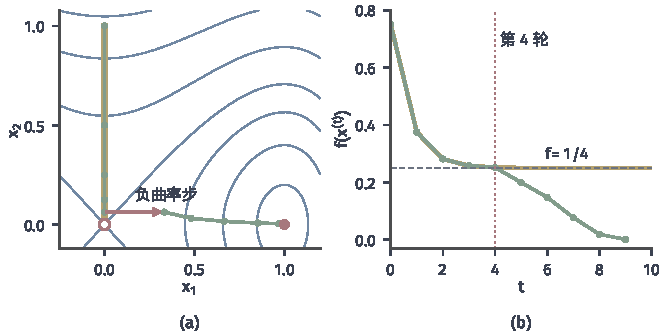
\includegraphics[width=112mm]{figures/05-optimization/02-smooth-optimization/matplotlib/saddle-nc-run/figure.pdf}
  \caption{从$(0,1)$出发的运行，步长$\alpha=1/2$。(a)绿色折线是梯度步与负曲率步的路径，红色箭头是第$4$轮的负曲率步，黄线（被绿线部分遮挡）是梯度下降，沿$x_2$轴收敛到空心点所示的鞍点。(b)目标值随轮数的变化，黄线趋于虚线$f=1/4$，绿线在红色点线所示的第$4$轮之后继续下降。}
  \label{fig:saddle-nc-run}
\end{BookInlineFigure}

\paragraph{算法分析}
每轮的下降都有下界，累加就得到轮数上界，论证与第~\ref{chap:smooth-foundations}章的累加下降相同。下面的定理把检测精度写成一个参数，以便同时覆盖精确和近似检测。

\begin{theorem}[交替算法的轮数]
 \label{thm:saddle-nc-count}
 设$f$有下界$f_{\inf}$，$\nabla f$和$\nabla^2f$在包含各步线段的凸集上分别是$L$-Lipschitz和$M$-Lipschitz的。设每次走负曲率步时都有$\gamma^{(t)}\geq\gamma_0>0$，记$\Delta_f=f(\bm{x}^{(0)})-f_{\inf}$。则算法~\eqref{eq:saddle-nc-update}停止之前的轮数$T$满足
 \begin{equation}
  T\leq\Delta_f\max\Bigl\{\frac{2L}{\varepsilon_g^2},\ \frac{3M^2}{2\gamma_0^3}\Bigr\}.
  \label{eq:saddle-nc-count}
 \end{equation}
\end{theorem}

\begin{proof}
 由下降引理，走梯度步的轮次下降至少$\lVert\bm{g}^{(t)}\rVert_2^2/(2L)$，而这些轮次$\lVert\bm{g}^{(t)}\rVert_2>\varepsilon_g$，下降超过$\varepsilon_g^2/(2L)$。

 由定理~\ref{thm:saddle-nc-step}，走负曲率步的轮次下降至少$2\gamma_0^3/(3M^2)$。记两者中较小的为$c$，累加$T$轮得
 \[
  \Delta_f\geq f(\bm{x}^{(0)})-f(\bm{x}^{(T)})\geq Tc.
 \]
 除以$c$即得式~\eqref{eq:saddle-nc-count}。
\end{proof}

例中$\Delta_f=3/4$。精确检测对应$\gamma_0=\varepsilon_H$，两项分别是$400$和约$116$，上界是$300$轮，实际只用了$9$轮。这也是一个最坏情形的界，它只用到$L$、$M$、$\Delta_f$，没有用到例子的具体形状。

\paragraph{适用范围}
这个算法要求能算出负曲率方向，在第~\ref{sec:saddle-detection}节的意义下，检测是确定的或者带失败概率的，第~\ref{sec:saddle-stopping}节再把这部分成本计入。定理只保证算法在有限步内停止，停止时的点满足两个容差，它不说明这个点是局部极小点。Hessian不是Lipschitz连续时，式~\eqref{eq:saddle-cubic}没有依据，步长公式也就失去了基础。

\subsection{扰动梯度法}
\label{sec:saddle-perturbed}

现在假设只能读取梯度，连Hessian向量积也不用。梯度下降在鞍点附近究竟怎样运动，是分析的起点。

\paragraph{鞍点附近的线性运动}
设$\bm{x}^\star$是严格鞍点，$\bm{H}=\nabla^2f(\bm{x}^\star)$。在$\bm{x}^\star$附近$\nabla f(\bm{x})\approx\bm{H}(\bm{x}-\bm{x}^\star)$，梯度下降近似于线性迭代：
\begin{equation}
 \bm{x}^{(t+1)}-\bm{x}^\star\approx(\bm{I}-\alpha\bm{H})\bigl(\bm{x}^{(t)}-\bm{x}^\star\bigr).
 \label{eq:saddle-linear}
\end{equation}

沿特征向量$\bm{q}_i$的分量每步乘以$1-\alpha\lambda_i$。$\alpha=1/L$时，正曲率方向的因子在$[0,1)$内，分量收缩；负曲率方向的因子$1+\alpha\lvert\lambda_i\rvert$大于$1$，分量放大。这正是第~\ref{sec:saddle-detection}节的幂迭代：梯度下降本身就在放大最负的方向。

例中两个坐标的迭代是
\[
 x_1^{(t+1)}=\frac32x_1^{(t)}-\frac12\bigl(x_1^{(t)}\bigr)^3,\qquad
 x_2^{(t+1)}=\frac12x_2^{(t)}.
\]
在原点附近，$x_1$每步约乘以$1.5$，$x_2$每步乘以$0.5$。图~\ref{fig:saddle-gd-linear}(b)的对数坐标下，两者都是直线，直到$x_1$接近$1$才不再增长。

\begin{BookInlineFigure}
  \centering
  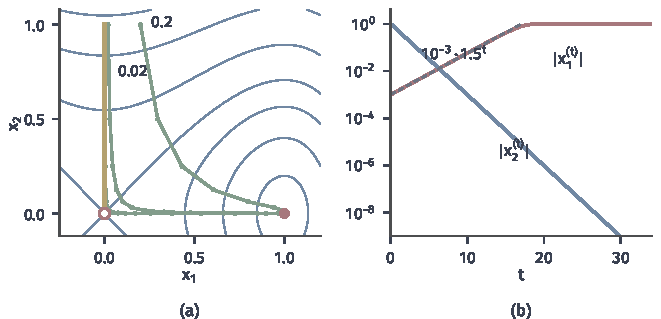
\includegraphics[width=112mm]{figures/05-optimization/02-smooth-optimization/matplotlib/saddle-gd-linear/figure.pdf}
  \caption{目标~\eqref{eq:saddle-example}上步长$1/2$的梯度下降。(a)从$(s,1)$出发的路径，绿线$s=0.2,0.02,0.002$，黄线$s=0$沿$x_2$轴收敛到鞍点。$s$越小，路径越贴近鞍点，徘徊越久。(b)从$(10^{-3},1)$出发，$\lvert x_1^{(t)}\rvert$（红）按$1.5^t$增长（灰色虚线），$\lvert x_2^{(t)}\rvert$（蓝）按$0.5^t$衰减。}
  \label{fig:saddle-gd-linear}
\end{BookInlineFigure}

\paragraph{什么样的初值会收敛到鞍点}
例中只要$x_1^{(0)}\neq0$，这个分量迟早被放大；只有$x_1^{(0)}=0$的点才一直留在$x_2$轴上，收敛到鞍点。这条轴是鞍点的\term{稳定流形}（stable manifold），二维平面上它的面积为零。

这个观察有严格的版本：设$f$二阶连续可微，$\nabla f$全局$L$-Lipschitz，步长$0<\alpha<1/L$，初值的分布对Lebesgue测度绝对连续，则梯度下降收敛到严格鞍点的概率为零\scite{lee2016gradient}。证明需要把迭代写成微分同胚，再用中心稳定流形定理，篇幅较长，读者可查阅原文。

这个结论有三个限度。第一，它的随机性只来自初值，之后的迭代完全确定。第二，它只排除收敛到严格鞍点，不说明会收敛到局部极小点，迭代也可能根本不收敛。第三，它是渐近的，没有说需要多少步。第三点不能靠更细的分析补上：要让$\lvert x_1\rvert$增长到$0.5$，例中的轮数如下。

\begin{BookInlineTable}
  \centering
  \begin{tabular}{@{}ccccc@{}}
    \toprule
    $x_1^{(0)}$ & $10^{-3}$ & $10^{-6}$ & $10^{-9}$ & $10^{-12}$\\
    \midrule
    轮数 & $16$ & $33$ & $50$ & $67$\\
    \bottomrule
  \end{tabular}
  \caption{目标~\eqref{eq:saddle-example}上$\lvert x_1^{(t)}\rvert$首次达到$0.5$所需的轮数。}
  \label{tab:saddle-escape-time}
\end{BookInlineTable}

初值的$x_1$可以任意接近零，轮数就可以任意大。所以普通梯度下降没有一个对所有初值都成立的有限步上界。要得到有限步的保证，必须让算法自己把迭代点推离稳定流形。

\paragraph{主要思想：只需要一点扰动}
图~\ref{fig:saddle-stuck-band}用数值实验看这件事。以原点为中心取半径$0.25$的圆盘，把每个点作为初值运行若干步梯度下降，再标出目标没有下降足够多的初值。这些“卡住”的初值组成一条沿$x_2$方向的窄带，步数越多，窄带越窄。

\begin{BookInlineFigure}
  \centering
  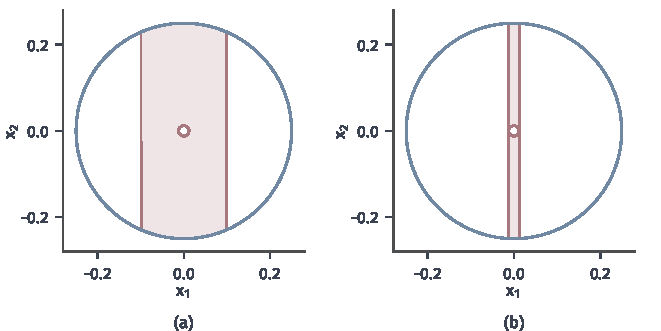
\includegraphics[width=112mm]{figures/05-optimization/02-smooth-optimization/matplotlib/saddle-stuck-band/figure.pdf}
  \caption{从半径$0.25$的圆盘（蓝线）内出发的梯度下降，步长$1/2$。红色窄带内的初值在$T$步后仍有$f>1/4-0.05$。(a)$T=3$，带的半宽约$0.099$。(b)$T=8$，带的半宽约$0.013$。窄带以外的点都已离开鞍点。}
  \label{fig:saddle-stuck-band}
\end{BookInlineFigure}

因此，在鞍点附近的小球内随机选一个点，落在窄带里的概率很小。图~\ref{fig:saddle-perturb-band}是概率的几何含义：窄带的体积与整个球的体积之比。只要球内的点几乎都能离开，加一点随机扰动就够了，扰动不需要很大。

\begin{BookInlineFigure}
  \centering
  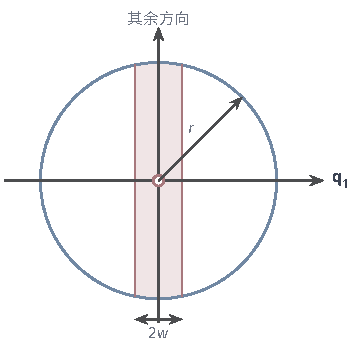
\includegraphics[width=61mm]{figures/05-optimization/02-smooth-optimization/tikz/saddle-perturb-band/figure.pdf}
  \caption{半径$r$的球内，沿$\bm{q}_1$方向半宽$w$的窄带。均匀随机的扰动落入窄带的概率就是两者的体积比。窄带外的点在$\bm{q}_1$上的分量至少是$w$。}
  \label{fig:saddle-perturb-band}
\end{BookInlineFigure}

先在二次目标上把这件事算清楚，此时$\bm{x}^\star$处的线性近似~\eqref{eq:saddle-linear}是精确的，全部论证都能写出来。

\begin{theorem}[二次目标上的逃离]
 \label{thm:saddle-quadratic-escape}
 设$f(\bm{x})=\tfrac12\bm{x}^\top\bm{H}\bm{x}$，$\bm{H}\in\mathbb{R}^{n\times n}$对称，$\lVert\bm{H}\rVert_2\leq L$，$\lambda_{\min}(\bm{H})=-\gamma<0$。$\bm{x}^{(0)}$在半径$r$的球内均匀分布，按步长$1/L$作梯度下降，迭代矩阵是$\bm{I}-\bm{H}/L$。给定$F>0$，$\delta\in(0,1)$，若
 \begin{equation}
  T\geq\frac{L}{\gamma}\ln\frac{4n\,(Lr^2+2F)}{\pi\gamma\,\delta^2r^2},
  \label{eq:saddle-quadratic-steps}
 \end{equation}
 则至少以$1-\delta$的概率，
 \begin{equation}
  f(\bm{x}^{(T)})\leq-F.
  \label{eq:saddle-quadratic-result}
 \end{equation}
\end{theorem}

\begin{proof}
 设$c_i=\langle\bm{x}^{(0)},\bm{q}_i\rangle$，$\bm{q}_1$对应$-\gamma$。证明分三步。

 第一步估计$c_1$不太小的概率。令$w>0$，事件$\lvert c_1\rvert\leq w$是球内半宽$w$的窄带，它的体积不超过宽度$2w$乘以$(n-1)$维截面的最大体积。记$V_m$为$m$维单位球的体积，于是
 \[
  \mathbb{P}\bigl(\lvert c_1\rvert\leq w\bigr)\leq\frac{2w\,r^{n-1}V_{n-1}}{r^nV_n}=\frac{2w}{r}\cdot\frac{V_{n-1}}{V_n}.
 \]

 单位球体积比由Gamma函数给出，再用Wendel不等式$\Gamma(x+\tfrac12)/\Gamma(x)\leq\sqrt{x}$，取$x=\tfrac{n+1}{2}$，得到
 \[
  \frac{V_{n-1}}{V_n}=\frac{\Gamma(\frac n2+1)}{\sqrt\pi\,\Gamma(\frac{n+1}{2})}\leq\sqrt{\frac{n+1}{2\pi}}\leq\sqrt{\frac{n}{\pi}}.
 \]

 取$w=\tfrac{r\delta}{2}\sqrt{\pi/n}$，窄带的概率不超过$\delta$。所以至少以$1-\delta$的概率，
 \[
  c_1^2\geq w^2=\frac{\pi\delta^2r^2}{4n}.
 \]

 第二步写出迭代的目标值。$\bm{x}^{(T)}$在$\bm{q}_i$上的分量是$(1-\lambda_i/L)^Tc_i$，所以
 \[
  f(\bm{x}^{(T)})=\frac12\sum_i\lambda_i\Bigl(1-\frac{\lambda_i}{L}\Bigr)^{2T}c_i^2.
 \]

 对$\lambda_i\geq0$的项，$0\leq1-\lambda_i/L\leq1$，这些项的和不超过$\tfrac12L\sum_ic_i^2\leq\tfrac12Lr^2$。对$\lambda_i<0$的项，它们都不大于零，只保留$\bm{q}_1$这一项，得到
 \[
  f(\bm{x}^{(T)})\leq\frac12Lr^2-\frac12\gamma\Bigl(1+\frac{\gamma}{L}\Bigr)^{2T}c_1^2.
 \]

 第三步确定步数。要使右端不超过$-F$，只需
 \[
  \Bigl(1+\frac{\gamma}{L}\Bigr)^{2T}\geq\frac{Lr^2+2F}{\gamma c_1^2}.
 \]

 由$\gamma\leq L$和不等式$\ln(1+y)\geq y/2$（$0\leq y\leq1$），左端的对数至少是$T\gamma/L$。代入$c_1^2$的下界，条件~\eqref{eq:saddle-quadratic-steps}恰好保证上式成立。
\end{proof}

定理把扰动的作用说清楚了。步数的主要部分是$L/\gamma$，即放大一倍需要的步数。维数$n$和失败概率$\delta$都在对数里，这是因为分量按指数增长，初值小一个倍数只增加常数步。高维时随机向量在任一方向上的分量约为$r/\sqrt n$，这个$\sqrt n$只通过$\ln n$进入步数。

例中在二次近似$\operatorname{diag}(-1,1)$上取$n=2$，$L=2$，$\gamma=1$，$r=0.05$，$F=0.05$，$\delta=0.1$，式~\eqref{eq:saddle-quadratic-steps}的右端约为$18.6$，所以$T=19$就够了。

图~\ref{fig:saddle-escape-scaling}用模拟检验定理。Hessian取$\operatorname{diag}(-\gamma,1,\ldots,1)$，其余参数同上，统计达到$f\leq-F$的步数。(a)中维数从$2$增加到$10^5$，中位数只从$7$增加到$20$。(b)中步数随$\gamma$减小按$1/\gamma$增长。上界比实际步数略大，但两种依赖关系都吻合。

\begin{BookInlineFigure}
  \centering
  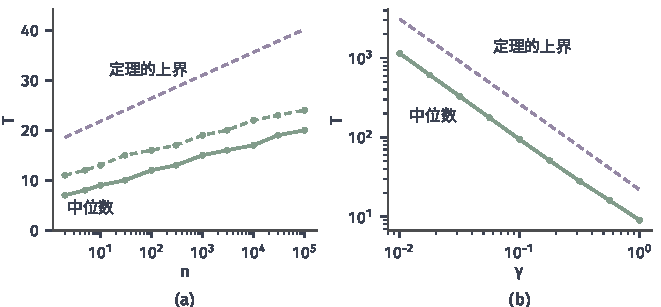
\includegraphics[width=112mm]{figures/05-optimization/02-smooth-optimization/matplotlib/saddle-escape-scaling/figure.pdf}
  \caption{二次目标上达到$f\leq-F$所需步数的模拟，每组$3000$次，$L=2$，$r=0.05$，$F=0.05$，Hessian取$\operatorname{diag}(-\gamma,1,\ldots,1)$。绿色实线是中位数，绿色虚线是$90\%$分位数，紫色虚线是式~\eqref{eq:saddle-quadratic-steps}在$\delta=0.1$时的上界。(a)$\gamma=1$，步数随维数$n$对数增长。(b)$n=10$，步数约与$1/\gamma$成正比。}
  \label{fig:saddle-escape-scaling}
\end{BookInlineFigure}

把上面的想法组成算法就是\term{扰动梯度法}（perturbed gradient method）：平时走梯度步；梯度小时加一次随机扰动，再运行一段固定长度的梯度步作为检验。目标下降了足够多，说明确实离开了鞍点，继续；否则就认为这里没有明显的负曲率，返回扰动之前的点。

\needspace{6\baselineskip}
\paragraph{变量}
算法要维护的量是：
\begin{itemize}
 \item $\bm{x}^{(t)}\in\mathbb{R}^n$，$\bm{g}^{(t)}\in\mathbb{R}^n$：当前点和梯度；
 \item $\tilde{\bm{x}}\in\mathbb{R}^n$，$\tilde f$：保存的基点及其目标值，这是可能返回的点；
 \item $\bm{\xi}\in\mathbb{R}^n$：扰动，在半径$r$的球内均匀抽取。
\end{itemize}

\paragraph{初始化}
选定起点、步长$\alpha=1/L$、梯度容差$\varepsilon_g$、扰动半径$r$、窗口长度$T_{\mathrm{w}}$和下降门槛$F$。例中沿用上面算出的$T_{\mathrm{w}}=19$，
\[
 \bm{x}^{(0)}=\begin{bmatrix}0\\1\end{bmatrix},\quad
 \varepsilon_g=0.1,\quad r=0.05,\quad F=0.05.
\]

\paragraph{每轮更新}
算法反复执行以下步骤，直到第$4$步返回。

\begin{enumerate}
 \item 计算$\bm{g}^{(t)}$。若$\lVert\bm{g}^{(t)}\rVert_2>\varepsilon_g$，走一步梯度步并回到第$1$步。例中与上一小节的前四轮相同，得到下面的点，它的梯度范数$0.0625$低于容差：
 \[
  \bm{x}^{(4)}=\begin{bmatrix}0\\0.0625\end{bmatrix}.
 \]
 \item 保存当前点为基点$\tilde{\bm{x}}$，记下它的目标值$\tilde f$，抽取$\bm{\xi}$，令当前点为$\tilde{\bm{x}}+\bm{\xi}$。例中设抽到$\bm{\xi}=(0.03,-0.02)$，于是
 \[
  \tilde f\approx0.2520,\qquad\tilde{\bm{x}}+\bm{\xi}=\begin{bmatrix}0.03\\0.0425\end{bmatrix}.
 \]
 \item 从这里开始连续走$T_{\mathrm{w}}$步梯度步。例中$x_1$的前几步是
 \[
  0.03,\ 0.0450,\ 0.0674,\ 0.101,\ 0.151,\ 0.225,\ 0.331,\ 0.479,\ 0.664,
 \]
 $x_2$每步减半，第$19$步后到达$(1.000,0.000)$，目标约为$10^{-15}$。
 \item 若窗口结束时目标比$\tilde f$下降了至少$F$，继续回到第$1$步；否则返回$\tilde{\bm{x}}$。例中第一次窗口下降了约$0.252\geq0.05$，继续。
\end{enumerate}

这时梯度范数约为$10^{-7}$，再次低于容差，于是在$(1,0)$处第二次扰动。为了便于比较，设仍抽到同一个$\bm{\xi}$，窗口结束时目标同样约为零，下降量远小于$F$，算法返回基点$\tilde{\bm{x}}\approx(1,0)$。整个过程用了$44$次梯度：起始$5$次，两个窗口各$19$次，第一个窗口结束时的判断$1$次。

图~\ref{fig:saddle-pgd-run}画出了这次运行。第一次窗口把迭代点从鞍点带到谷底，第二次窗口只用来确认谷底附近没有可以利用的负曲率。这也说明了成本的构成：确认“没有”和发现“有”花费相同的$T_{\mathrm{w}}$步。

\begin{BookInlineFigure}
  \centering
  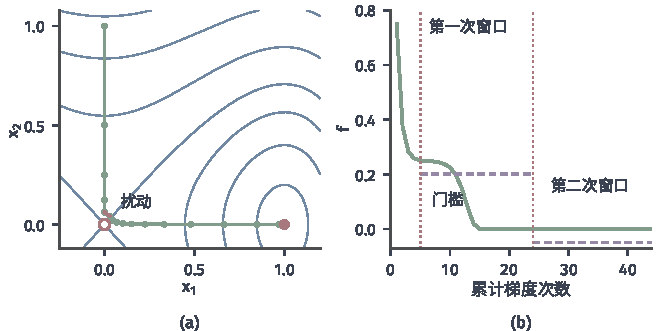
\includegraphics[width=112mm]{figures/05-optimization/02-smooth-optimization/matplotlib/saddle-pgd-run/figure.pdf}
  \caption{扰动梯度法在目标~\eqref{eq:saddle-example}上的运行，$T_{\mathrm{w}}=19$，$F=0.05$，$\bm{\xi}=(0.03,-0.02)$。(a)绿线是路径，红色短线是扰动。(b)目标值随累计梯度次数的变化，红色点线是触发扰动的时刻，紫色虚线是各窗口要求达到的门槛。第一次窗口越过门槛，第二次窗口没有。}
  \label{fig:saddle-pgd-run}
\end{BookInlineFigure}

\paragraph{一般目标上的保证}
定理~\ref{thm:saddle-quadratic-escape}只对二次目标成立。目标不是二次时，Hessian会随位置变化，放大过程可能被打断，所以需要Hessian的Lipschitz条件来控制窗口内的偏差。参数按下面的方式联合选取时，有如下保证\scite{jin2017escape}。

\begin{theorem}[扰动梯度法的高概率保证]
 \label{thm:saddle-pgd}
 设$f$下有界，$\nabla f$是$L$-Lipschitz的，$\nabla^2f$是$M$-Lipschitz的，$\Delta_f=f(\bm{x}^{(0)})-f_{\inf}$，$\varepsilon\leq L^2/M$。取$\alpha=1/L$，半径$r$、窗口$T_{\mathrm{w}}$和门槛$F$按$L,M,\varepsilon,\delta,n,\Delta_f$确定，则至少以$1-\delta$的概率，扰动梯度法返回的点满足
 \begin{equation}
  \lVert\nabla f(\tilde{\bm{x}})\rVert_2\leq\varepsilon,\qquad
  \lambda_{\min}\bigl(\nabla^2f(\tilde{\bm{x}})\bigr)\geq-\sqrt{M\varepsilon},
  \label{eq:saddle-pgd-guarantee}
 \end{equation}
 所用梯度次数为$\tilde O\bigl(L\Delta_f/\varepsilon^2\bigr)$，$\tilde O$隐去了$n,1/\delta,L,M,\Delta_f,1/\varepsilon$的多项对数因子。
\end{theorem}

证明的核心比二次情形多了一个技巧。不能再按特征分量独立讨论，于是考虑两条从窄带两侧出发、只在$\bm{q}_1$方向相差$2w$的迭代序列，用Hessian的Lipschitz条件证明它们的差在窗口内按指数增长，因此两条序列至少有一条离开基点足够远，目标也因此下降足够多。这说明“卡住”的初值不可能在$\bm{q}_1$方向上有大于$2w$的宽度，窄带的宽度得到了控制。完整论证篇幅较长，读者可查阅\scite{jin2017escape}。

定理对参数的要求是实质性的。扰动半径、窗口长度和门槛必须与$L$、$M$、$\varepsilon$和目标下降总量匹配。这里要区分两件事：结论说的是以高概率到达式~\eqref{eq:saddle-pgd-guarantee}定义的点，而不是找到局部极小点，更不是全局最优解。

\paragraph{严格鞍点的结论不能搬到退化驻点}
上面的论证依赖指数放大。退化驻点上没有负特征值，放大是多项式的。比较两个一元函数，步长取$\alpha=\tfrac12$：
\[
 -\frac12y^2:\quad y^{(t+1)}=\frac32y^{(t)};\qquad
 -\frac14y^4:\quad y^{(t+1)}=y^{(t)}+\frac12\bigl(y^{(t)}\bigr)^3.
\]

前者每步放大常数倍，从$y^{(0)}$到$0.5$只要$\log_{1.5}(0.5/y^{(0)})$步。后者可以用微分方程估计：$\mathrm{d}y/\mathrm{d}t\approx\tfrac12y^3$给出$1/y^2$随$t$线性减小，所需步数约为$1/(y^{(0)})^2$。从$y^{(0)}=0.01$出发，两者的实际步数分别是$10$和$10002$。图~\ref{fig:saddle-degenerate-escape}比较了这两种依赖。

\begin{BookInlineFigure}
  \centering
  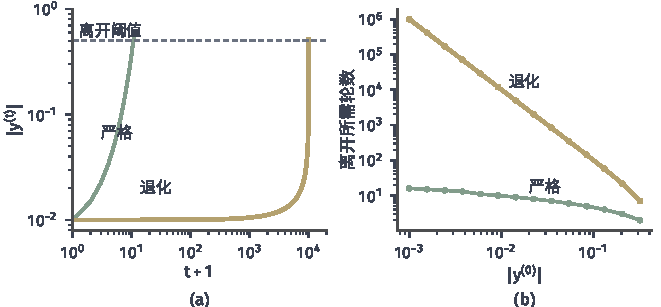
\includegraphics[width=112mm]{figures/05-optimization/02-smooth-optimization/matplotlib/saddle-degenerate-escape/figure.pdf}
  \caption{严格鞍点（绿，$-y^2/2$）与退化驻点（黄，$-y^4/4$）上步长$1/2$的梯度下降。(a)从$y^{(0)}=0.01$出发的$\lvert y^{(t)}\rvert$，虚线是离开阈值$0.5$。(b)离开所需轮数随初值大小的变化，严格鞍点按对数增长，退化驻点按$1/(y^{(0)})^2$增长。}
  \label{fig:saddle-degenerate-escape}
\end{BookInlineFigure}

在一个由$x_1^2-x_2^4$描述的退化鞍点上，扰动梯度法的窗口$T_{\mathrm{w}}$按严格鞍点设计，时间内分量几乎不长，窗口结束时目标没有明显下降，算法就返回基点。这并不违反定理~\ref{thm:saddle-pgd}：基点的$\lambda_{\min}=0\geq-\sqrt{M\varepsilon}$，它满足定理宣称的条件，只是这个条件本来就不排除退化鞍点。

\subsection{利用非正定模型}
\label{sec:saddle-indefinite-model}

二阶方法手里本来就有曲率矩阵。第~\ref{chap:second-order-methods}章和第~\ref{chap:trust-region}章对不定矩阵采取了两种态度：前者把矩阵修正成正定的，后者保留矩阵原样，用半径把模型关起来。这里比较两种态度在鞍点附近的差别，特别是哪种能利用负曲率。

\paragraph{信赖域模型怎样使用负曲率}
回顾第~\ref{chap:trust-region}章的子问题：
\begin{equation}
 \min_{\lVert\bm{p}\rVert_2\leq\Delta}\ m(\bm{p})=f(\bm{x})+\langle\bm{g},\bm{p}\rangle+\frac12\bm{p}^\top\bm{B}\bm{p}.
 \label{eq:saddle-tr-subproblem}
\end{equation}
$\bm{p}$是全局解的充要条件是存在$\lambda\geq0$，使
\begin{equation}
 (\bm{B}+\lambda\bm{I})\bm{p}=-\bm{g},\qquad
 \bm{B}+\lambda\bm{I}\succeq\bm{0},\qquad
 \lambda\bigl(\Delta-\lVert\bm{p}\rVert_2\bigr)=0.
 \label{eq:saddle-tr-optimality}
\end{equation}

第二个条件说明$\lambda\geq-\lambda_{\min}(\bm{B})$。所以$\bm{B}$不定时$\lambda>0$，解一定在边界上：模型沿负曲率方向一直下降，直到碰上半径。这里没有把任何曲率改成正值，负曲率被直接转化成一个长度为$\Delta$的步。

在原点取$\bm{B}=\operatorname{diag}(-1,1)$，$\Delta=\tfrac12$，$\bm{g}=\bm{0}$。条件~\eqref{eq:saddle-tr-optimality}给出$\lambda=1$，第一个方程$(\bm{B}+\bm{I})\bm{p}=\bm{0}$只约束$p_2=0$，于是
\[
 \bm{p}=\begin{bmatrix}\pm\tfrac12\\0\end{bmatrix},\qquad
 m(\bm{0})-m(\bm{p})=\frac18.
\]

代回目标，实际下降和两者之比分别是
\[
 f(\bm{0})-f\bigl(\tfrac12,0\bigr)=\frac14-\frac{9}{64}=0.1094,\qquad
 \rho=\frac{0.1094}{0.125}\approx0.875.
\]
这一步可以接受。梯度精确为零，信赖域仍然走出了一大步，这是只靠梯度的方法做不到的。

\paragraph{修正Hessian的用途不同}
第~\ref{chap:second-order-methods}章的修正让矩阵变成$\bm{B}=\bm{H}+\bm{E}\succ\bm{0}$，解$\bm{B}\bm{d}=-\bm{g}$，目的是得到下降方向，让线搜索有效。这时$\bm{g}=\bm{0}$意味着$\bm{d}=\bm{0}$，算法原地不动。

$\bm{g}$很小但不为零时，以谱修正为例，方向沿$\bm{q}_i$的分量是$-\langle\bm{g},\bm{q}_i\rangle/\lvert\lambda_i\rvert$，长度正比于梯度，鞍点附近很短。下面在点$(0.01,0.0625)$上比较两者。由式~\eqref{eq:saddle-example-derivatives}，该点的数据是
\[
 \bm{g}\approx\begin{bmatrix}-0.0100\\0.0625\end{bmatrix},\qquad
 \bm{H}\approx\operatorname{diag}(-0.9997,1).
\]

谱修正取绝对值，得到的方向和$\Delta=\tfrac12$时子问题的解分别是
\[
 \bm{d}\approx\begin{bmatrix}0.0100\\-0.0625\end{bmatrix},\qquad
 \bm{p}\approx\begin{bmatrix}0.4990\\-0.0309\end{bmatrix}.
\]

子问题的$\lambda\approx1.020$，预测下降$0.1309$，实际下降$0.1142$，$\rho\approx0.872$，接受。修正方向沿$x_1$的分量只有子问题解的约$2\%$。图~\ref{fig:saddle-tr-modified}(a)画出了这两个方向，(b)比较后续运行：修正方法配回溯时，$x_1$大约每轮翻一倍，要$6$轮才接近$0.77$；信赖域$3$轮之内就到了谷底附近，其间有一次拒绝。

\begin{BookInlineFigure}
  \centering
  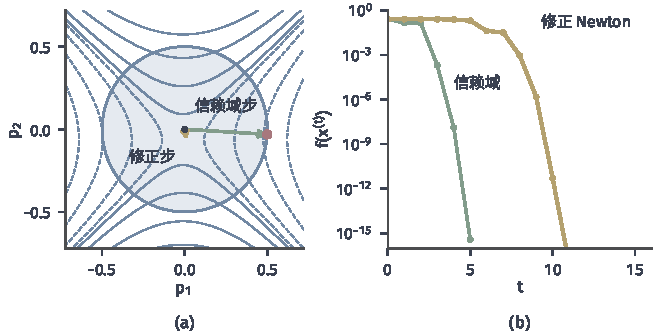
\includegraphics[width=112mm]{figures/05-optimization/02-smooth-optimization/matplotlib/saddle-tr-modified/figure.pdf}
  \caption{点$(0.01,0.0625)$处的比较。(a)蓝线是二次模型的等高线（虚线为负值），浅蓝圆盘半径$\Delta=1/2$，绿色箭头指向子问题的解（红点），黄色短箭头是谱修正方向。(b)从该点出发目标值随轮数的变化，绿线是精确求解子问题的信赖域，黄线是谱修正加Armijo回溯。}
  \label{fig:saddle-tr-modified}
\end{BookInlineFigure}

\paragraph{梯度与负曲率方向正交时}
最能说明两种方法差别的是$\langle\bm{g},\bm{q}_1\rangle=0$的情形。在点$(0,0.0625)$，梯度是$(0,0.0625)$，与$\bm{e}_1$正交。此时条件~\eqref{eq:saddle-tr-optimality}的第一行变成$(\lambda-1)p_1=0$，半正定条件要求$\lambda\geq1$。取$\lambda=1$，第二行和球面条件给出
\[
 p_2=-\frac{0.0625}{1+1}=-0.03125,\qquad
 p_1=\pm\sqrt{\Delta^2-p_2^2}\approx\pm0.4990.
\]

这是第~\ref{chap:trust-region}章所说的困难情形：$\bm{B}+\lambda\bm{I}$奇异，方程本身不能确定$p_1$，要沿$\bm{q}_1$方向补一个分量才到达边界。这一步的预测下降是$0.1260$，$\rho\approx0.877$。

截断共轭梯度却看不到$\bm{e}_1$。它的迭代只在由$\bm{g}$生成的Krylov子空间中进行，这里就是$x_2$轴，第一步就到达$(0,-0.0625)$，残差为零而停止，预测下降只有约$0.002$。图~\ref{fig:saddle-tr-hard-case}(a)是这个点上的模型，(b)是从$(0,1)$出发的运行。截断共轭梯度第一步到达原点，$\bm{g}=\bm{0}$，算法宣布完成。精确子问题第一步是$(0.866,-0.5)$，比值$\rho=0.8125$，第二步到达$(1.039,0)$。

\begin{BookInlineFigure}
  \centering
  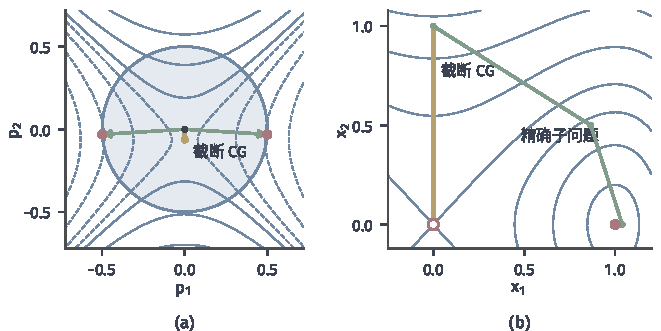
\includegraphics[width=112mm]{figures/05-optimization/02-smooth-optimization/matplotlib/saddle-tr-hard-case/figure.pdf}
  \caption{困难情形。(a)点$(0,0.0625)$处的模型（蓝线）与半径$1/2$的圆盘，两个红点是子问题的全局解，黄线是截断共轭梯度的结果，它留在$p_2$轴上。(b)从$(0,1)$出发、$\Delta^{(0)}=1$的运行：绿线精确求解子问题，黄线用截断共轭梯度，一步到达鞍点后停止。}
  \label{fig:saddle-tr-hard-case}
\end{BookInlineFigure}

这里要记住：算出的步是否利用负曲率，由子问题的求解方式决定。使用截断共轭梯度的信赖域，在$\bm{g}$恰好避开$\bm{q}_1$时和修正方法一样看不见负曲率。

\paragraph{后续保证的差别}
第~\ref{chap:trust-region}章的二阶保证要求候选步的模型下降满足下面的条件，其中$\lambda_-=\max\{0,-\lambda_{\min}\}$，$c_2>0$是常数：
\[
 \operatorname{pred}(\bm{p})\geq c_2\lambda_-\Delta^2.
\]
由此得到
\begin{equation}
 \liminf_{t\to\infty}\max\bigl\{\lVert\bm{g}^{(t)}\rVert_2,\ \lambda_-^{(t)}\bigr\}=0.
 \label{eq:saddle-tr-liminf}
\end{equation}
精确解$c_2=\tfrac12$，满足这一条；只有一阶信息的步不满足，保证也就退回到$\bm{g}^{(t)}\to\bm{0}$。

不想精确求解时，可以把第~\ref{sec:saddle-detection}节的检测嫁接进来。设检测给出$\bm{v}$，$\bm{v}^\top\bm{B}\bm{v}\leq-\gamma$，选符号使$\langle\bm{g},\bm{v}\rangle\leq0$，把$\Delta\bm{v}$作为候选步，它的预测下降是
\[
 m(\bm{0})-m(\Delta\bm{v})=-\Delta\langle\bm{g},\bm{v}\rangle-\frac{\Delta^2}{2}\bm{v}^\top\bm{B}\bm{v}\geq\frac12\gamma\Delta^2.
\]

只要$\gamma$不小于$\lambda_-$的一个固定倍数，例如$\gamma\geq\tfrac12\lambda_-$，就得到$c_2=\tfrac14$，第~\ref{chap:trust-region}章的论证可以照搬。当然这样一来保证就带上了检测的失败概率。表~\ref{tab:saddle-model-compare}总结了各种做法的区别。

\begin{BookInlineTable}
  \centering
  \begin{tabular}{@{}lll@{}}
    \toprule
    做法 & 在$\bm{g}=\bm{0}$的鞍点 & 结论\\
    \midrule
    修正Hessian加线搜索 & 不动 & $\bm{g}^{(t)}\to\bm{0}$\\
    信赖域，Cauchy步或截断CG & 不动 & $\bm{g}^{(t)}\to\bm{0}$\\
    信赖域，精确子问题 & 走到边界 & 式~\eqref{eq:saddle-tr-liminf}\\
    信赖域，加入负曲率检测 & 走到边界 & 同上，带失败概率\\
    \bottomrule
  \end{tabular}
  \caption{几种处理不定矩阵的做法。式~\eqref{eq:saddle-tr-liminf}的二阶结论只说明子列满足二阶必要条件，不说明极限点是局部极小点。}
  \label{tab:saddle-model-compare}
\end{BookInlineTable}

总之，修正Hessian解决的是“方向要下降”，保留不定模型解决的是“负曲率要被利用”。两者的出发点不同，后续能给出的保证也不同，不应混为一谈。

